\chapter{Cuantización}

La cuantización, como ya definimos en el apartado \ref{cap:cuantización}, se trata de un proceso por el cual tomamos un modelo entrenado para arquitecturas de escritorio de la forma habitual, y realizamos una serie de operaciones de simplificación o transformaciones del formato numérico para obtener un modelo cuyos requisitos de espacio y tiempos de inferencia se ven reducidos considerablemente. 

Este procedimiento es el núcleo del proyecto, y el objetivo real de estudio de modelos para tecnologías móviles: experimentar cuál es la diferencia en tiempo y uso de memoria de la arquitectura tradicional sobre la optimizada.

Para realizar este proceso, emplearemos la API de Pytorch dedicada a la transformación e implementación de modelos convolucionales en Android: Pytorch mobile  \cite{pmobile}. En este punto, analizaremos las optimizaciones realizadas por este framework, y las ventajas y desventajas de dicho procedimiento.

\section{Optimizaciones de Pytorch mobile}
\subsection{Capacidades del framework}
Pytorch, a través de sus dependecias mobile, puede transformar en unos sencillos pasos un modelo entrenado con Pytorch a un modelo simplificado optimizado para dispositivos móviles. Incluye varios métodos relacionados con la exportación que permiten optimizar o no la salida del modelo, adecuándolo a nuestras necesidades. En su página oficial, podemos encontrar un grafo donde se describe este proceso \cite{pmobile}:

\begin{figure}[H]
	\centering
	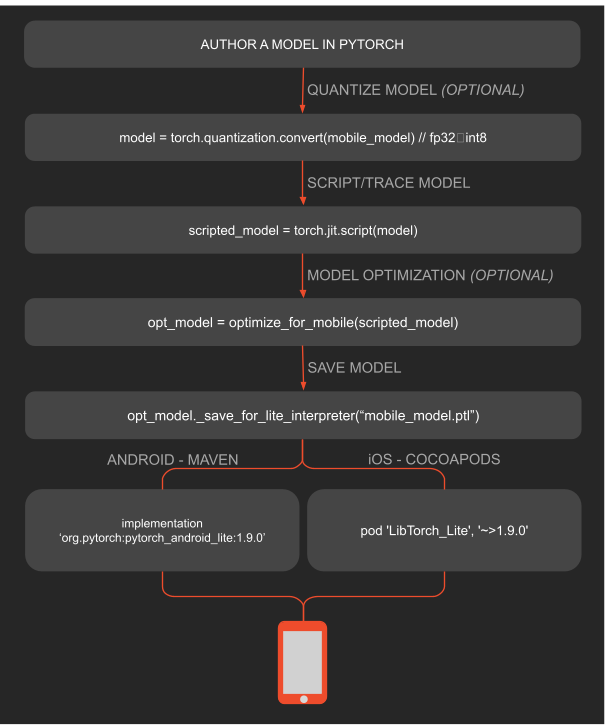
\includegraphics[scale = 0.6]{imagenes/pytorch-mobile.png}
	\caption{Optimización de modelos con Pytorch Mobile \cite{pmobile}}
	\label {fig:mobileprocess}
\end{figure}

Su compatibilidad engloba Android y iOS, siendo este último sistema soportado oficialmente tras el comienzo de la realización de este TFG. Aun así, este proyecto fue concebido inicialmente para ser probado en dispositivos Android, ya que el hardware de estos dispositivos tiene un mayor rendimiento en CPU y GPU, así como un mejor soporte de las librerías de aprendizaje. iOS, al tratarse de un SO cerrado a dispositivos Apple, y difícilmente emulable si no se dispone de dispositivos de la marca, requiere aún la existencia de frameworks estables dedicados al aprendizaje. Este motivo, sumando a que no disponemos de dispositivos con este sistema operativo, inclinó la balanza a usar únicamente dispositivos Android como dispositivo objetivo.

\subsection{Optimizaciones disponibles}

Pytorch mobile dispone para Android de una lista de 5 optimizaciones posibles a realizar sobre el modelo. Todas ellas, seleccionables de forma independiente, o aplicadas en conjunto por defecto, cubren los siguientes aspectos:

\begin{itemize}
	\item Fusión de las capa de convolución y normalización de batch: realiza una integración de los valores de normalización dentro de la capa convolutiva, ya que no será necesario reajustar esos valores para inferencia-
	\item Inserción y plegado de operaciones: utiliza la librería XNNPack, que se trata de un sistema de operaciones en coma flotante especialmente optimizado para ARM, que permite variar la precisión de los valores flotantes según el modelo. Fusiona las operaciones lineales y de convolución, de forma que se realicen en un menor tiempo.
	\item Fusión de la función ReLu con el conjunto de operaciones empaquetado creado con XNNPack en el paso anterior.
	\item Eliminación del dropout, ya que en tiempo de inferencia, se busca el mejor resultado si necesidad de reentreno.
	\item Optimización del grafo interno del modelo correspondiente a la convolución, para hacer que formen parte de un solo bloque raiz y mejore el tiempo de inferencia.	
\end{itemize}

En total, la web  \cite{pmobile} estima una ganancia aproximada del 60\% en tiempo de inferencia de forma teórica. Sin embargo, este valor puede oscilar en función de los datos que se estén evaluando, la arquitectura que deseamos cuantizar, y las capacidades de cálculo del dispositivo objetivo. A continuación, estudiaremos los resultados ofrecidos, y si merece la pena la aplicación de este proceso.

\section{Creación de los modelos cuantizados}

La transformación de los modelos entrenados a su versión cuantizada puede realizarse de forma inmediata, ya que en los pasos anteriores, el modelo entrenado sobre cada uno de los casos (clasificación binaria, y multiclase para benigno y maligno) fue almacenado en un fichero de formato .pt (extensión de modelo Pytorch).

Al tratarse de una conversión post-entrenamiento, no se requiere ningún ajuste de parámetros previo durante el entrenamiento, lo cual significa el entrenamiento sobre los modelos preparados para cuantización (QAT, o Quantization Aware Training  \cite{kuzmin2024fp8}), con el coste de una pequeña pérdida respecto a dicha ténica.

Para cuantizar el modelo tras su entrenamiento, basta con realizar los siguientes pasos:
\begin{enumerate}
	\item Cargar el modelo entrenado previamente. Como en nuestro caso, hemos realizado el salvado del modelo y procedemos a realizar la cuantización en el mismo en el mismo script, podemos directamente emplear el objeto Learner que almacena el modelo completo. En caso de que se quisiese leer de disco duro, bastaría con usar la función model.load().
	\item Activar el modo de evaluación del modelo. De esta forma, bloqueamos los parámetros libres de las capas de normalización de batches, y la aplicación de dropout.
	\item En este punto, podemos optar por dos opciones:
	\begin{enumerate}
		\item Exportar el modelo a Android sin ninguna optimización estructural, más allá de la adaptación de tipos de flotantes (función \textit{save\_for\_lite\_interpreter})
		\item Exportar el modelo aplicando todas las optimizaciones anteriores mencionadas para obtener el modelo más eficiente posible (función \textit{export\_for\_mobile})
	\end{enumerate}
	\item (Opcional) : exportar el modelo de escritorio en formato torch script. Se trata de un lenguaje de representación universal del modelo, que puede ser empleado con python nativo, y ser transferido a otros frameworks de trabajo habituales.
		
\end{enumerate}

Para realizar la comparativa de forma lo más exhaustiva posible, tomaremos el modelo de Android, y lo evaluaremos con el conjunto completo de imágenes de test, de forma que la valoración obtenida sea completamente representativa.

El pseucódigo resultante es batante sencillo, y su explicación queda prácticamente autocontenida gracias al uso de nombres de función represetativos:

\begin{algorithm}[H]
	\label{fig:cuantizado}
	\caption{Proceso de cuantizado de modelos a Android}
	\begin{algorithmic}
		\Procedure{exportar\_modelo}{learner: Learner Model Object, savename : String}
	
		\State model = learner.model.to('cpu') : Model
		\ State model.eval()
		
		 \State scripted\_module = torch.jit.script(nn.Sequential(model, Softmax(dim=n))) \\
		\Comment{Exportación del modelo original}
	 	 \State scripted\_module.save(savename + ``Full.pt")\\  
		 \Comment{Exportación del modelo optimizado}
		 \State optimized\_scripted\_module = optimize\_for\_mobile(scripted\_module) 
		 \State optimized\_scripted\_module.\_save\_for\_lite\_interpreter(savenameFull+ ``\_androidOptimized.pt")
	
		\EndProcedure
		
	\end{algorithmic}
\end{algorithm}

Podemos observar que el proceso es trivial, a excepción del último punto, donde se realiza la definición de un objeto de tipo sencuencial. Esto se debe que, cuando exportamos el modelo a Android, existen dos posibles alternativas para interpretar la capa de salida del mismo:
\begin{enumerate}
	\item Interpretando el tensor de salida de la función Softmax por columnas, de forma que la clase predicha para cada imagen será el máximo valor softmax encontrado en la columna en cuestión. En Python, se le conoce como máximo en dimensión 0, al tratarse del máximo de todas las filas.
	\item Interprentando el tensor de salida por filas, donde una imagen de entrenada recibe como etiqueta de salida el índice de la posición de fila cuyo valor es mayor. En este caso, se considera como dimensión 1, ya que se trata del valor máximo encontrado entre las columnas.
 \end{enumerate}

Por tanto, antes de exportar el modelo, será necesario especificar la dimensión de lectura. En versiones anteriores, esta dimensión era elegida de forma implícita por la función, pero ahora, debemos especificarla explícitamente para tener un correcto funcionamiento. Como en nuestro caso, solo tenemos una dimensión de etiquetas por modelos, debemos seleccionar el valor máximo por columnas, y valor a especificar es dim=1. Basta con crear un objeto de tipo Softmax, y especificar como parámetro \textit{dim}, el valor dim = 1.

Para concatenar el modelo original, y la nueva capa específica para la función Softmax, es necesario añadir ambos pasos a un pipeline, usando para la clase Sequential de Pytorch, que no es más que la creación de un modelo por capas.\\

\section{Comparativa de los modelos original y cuantizado}

En este apartado, una vez comprendido el proceso de exportación y cuantización, examinaremos el rendimiento de cada uno de los 3 modelos creados para el proyecto. Para ello, evaluaremos el conjunto de test, intacto hasta esta fase, para conocer el rendimiento real de los modelos originales, y los compararemos con cada uno de los modelos cuantizados.

\subsection{Cuantización del modelo binario}

El modelo de clasificación binaria, que decide si la enfermedad se trata de un caso benigno o maligno, es la capa más importante de la arquitectura de dos niveles implementada. Su rendimiento es crítico dentro del funcionamiento del modelo, debido a que la confusión entre subtipos de enfermedades tiene un coste relativamente pequeño, pero un error entre una enfermedad cancerígena o benigna tiene un elevado coste para el paciente en consecuencias. Por tanto, es clave evaluar el modelo con el conjunto de test para conocer la bonanza del mismo, y estudiar si las gancias en espacio y tiempo de inferencia justifican la cuantización.\\

Comenzaremos por evaluar el conjunto de test con el modelo original sin cuantizar, para tenerlo como referencia. Los resultados ofrecidos en accuracy, balanced accuracy, precision y recall son los siguientes:

